\section{Contexto de trabajo}

Actualmente vivimos en un entorno que dominado por la tecnología. Día a día se desarrollan nuevas herramientas con el fin de ayudar al ser humano a realizar tareas de una forma más fácil y eficiente, como los HMD (Head-mounted Display)\cite{B15}.
Por otro lado también nos encontramos en una época donde el diseño es un área de gran importancia en cualquier sector del mercado, por ejemplo, un buen diseño web en un sitio es fundamental lograr que un producto se logre vender o difundir, un buen diseño gráfico en campañas de marketing asegura más clientes; de igual forma nos encontramos con el diseño de interiores. Para ésta última área se suelen contratar diseñadores de interiores profesionales para lograr que los espacios interiores de un inmueble consigan tal armonía que mejoren la calidad de vida de quienes lo habitan y además generen un impacto en las personas que usan éstas habitaciones.\par
El proceso del diseño de interiores está integrado por varias etapas, que se pueden observar en la figura 1.1	.
Teniendo a la mano una gran diversidad de herramientas tecnológicas, podemos usar estos elementos para lograr que el diseño de interiores sea más sencillo, intuitivo y más rápido, y que cualquier persona pueda realizarlo sin tener todos los conocimientos y habilidades que se requieren para ello.

\begin{figure}[!h]
	\centering
	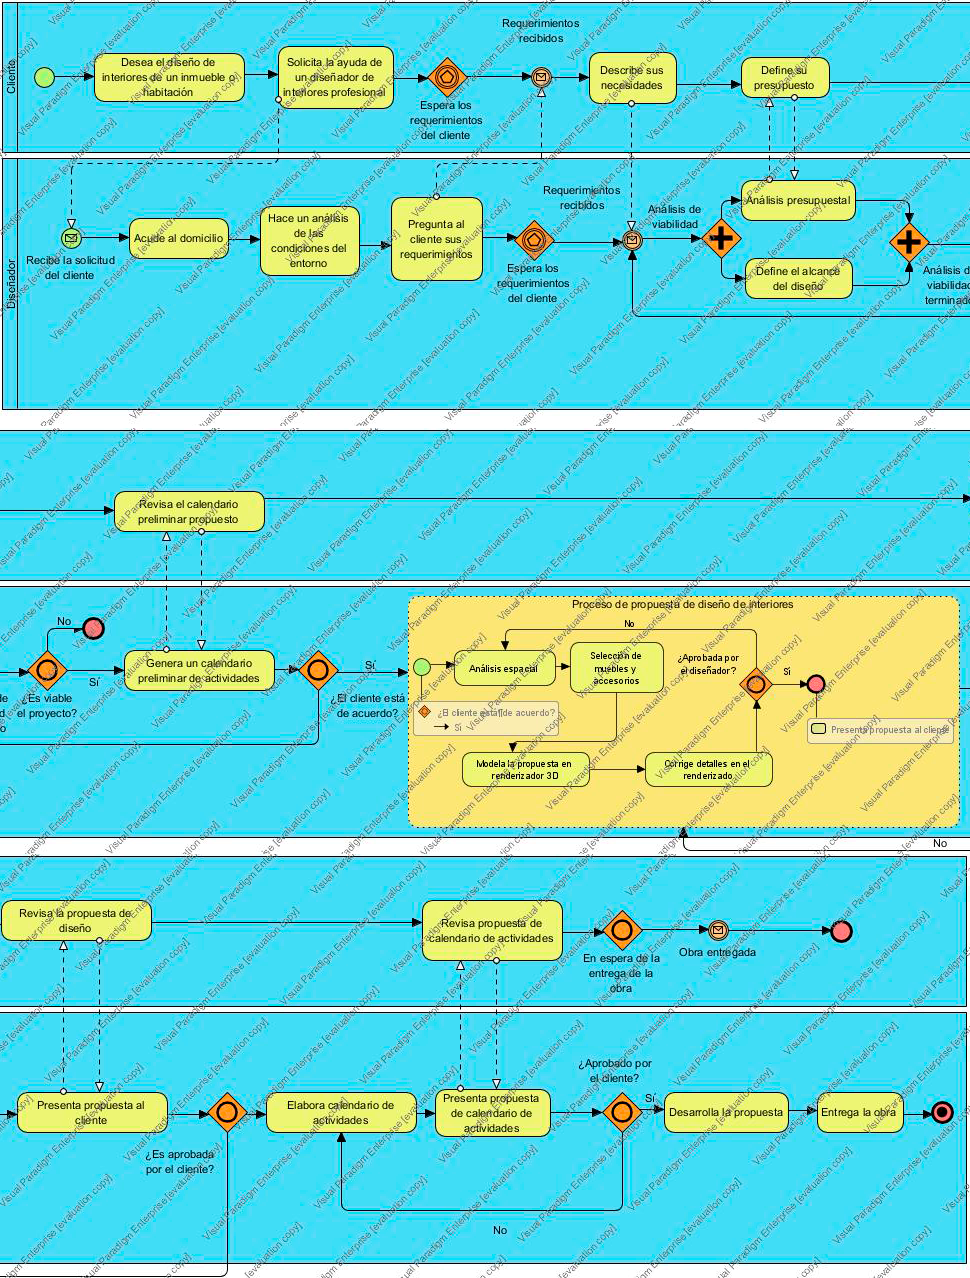
\includegraphics[width=17.5cm]{imagenes/marcoteorico/bpmn01.png}
	\caption{Modelo del proceso de diseño de interiores.}
	\label{fig:bpmn_antes}
\end{figure}